% ------------------------- MAIN TASK ---------------------------------
\section{Main task}
\subsection{Schematic proposal for limiting output current to 250mA} \label{ssec:num11}
{
	We were asked to design a proposed scheme to limit the output current to 250mA, to do this we decided to change the principle of the connections to create a current source using the LM317.	
	
	\begin{figure}[h]
		\centering
		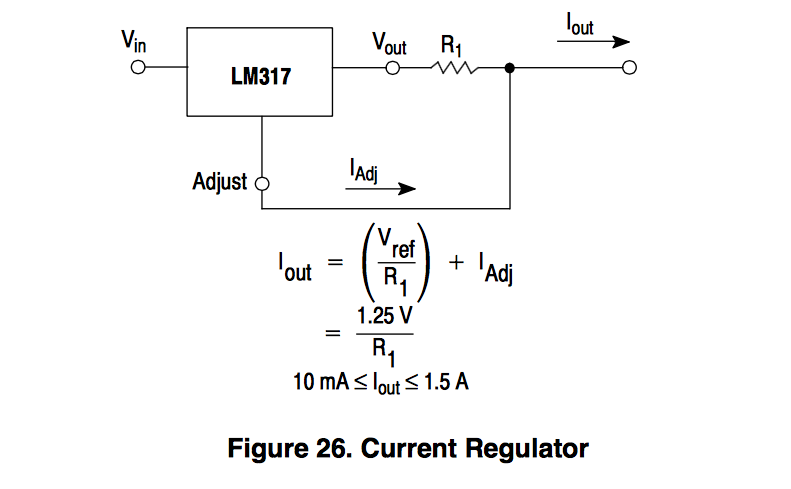
\includegraphics[width=0.7\linewidth]{../Figures/Partie2/SourceCourant}
		\caption{Current source with LM317}
		\source{Stackexchange "lm317-µa-constant-current-source-possibility"}
		\label{fig:sourcecourant}
	\end{figure}
	
	We use the reference voltage (\textbf{1.25V}) of the internal diode, so the output current depends on the resistance \textbf{R1} plus the leakage current of the diode.
	
	By adding and changing a load resistor in the circuit, the induced output current will vary, as will the voltage, but the current will not exceed : \\ $\frac{Vref}{R1}+I_{ADJ}$
	
	This 
	
}

\subsection{Plotting output tension depending on output current} \label{ssec:num12}
{}
\subsection{Oscillogram of the output current depending on the input tension} \label{ssec:num13}
{}
\subsection{Dissipated power calculation} \label{ssec:num14}
{}
\subsection{Estimation of the junction's temperature without cooling} \label{ssec:num15}
{}
\subsection{Short-circuited output - dissipated power calculation} \label{ssec:num16}
{}
\clearpage